% ==============================================================================
%
%                             Dataflow
%
% ==============================================================================
\chapter{Dataflow} \label{chapt:dataflow}
With the Wallis filter implemented on the FPGA the problem becomes that the
image data has to be sent from the computer to the FPGA and back. The following
chapter explains the realiztion of said dataflow. It is split into two main
parts: The communcation and control parts.

During the work on the project it was discovered that the initial approach to
the problem would not lead to the optimum solution. This is why a second
implementation was made that differs in both communication and control parts. To
prevent confusion these two solutions are refered to as solution A (the first
approach) and solution B (the second, more performant approach).

% ==============================================================================
%                             Communication
% ==============================================================================
\section{Communication}
The UFT core from project 5 serves as a starting point to the communication
problem. Altough it works on a fundamental basis, the following key features are
missing:

\begin{itemize}
	\item Acknowledgment of received data
	\item Retransmission if a packat was not received
	\item Control interface
	\item Stream based data interface
\end{itemize}

In the following chapters these four problems are addressed and the solutions
explained.

% ==============================================================================
%                             Acknowledge
% ==============================================================================
\subsection{Acknowledge}
The communication is based on the User Datagram Protocol (UDP). This protocol
features low overhead and is simple to implement. The main problem is that the
data sent is not acknowledged hence the sender has no feedback wheather the data
was received or not. This is one reason a custom session protocol (UFT: UDP
File Transfer) was introduced in project 5. It provides command packets for data
packet acknowledgment. Table \ref{tab:uftcommandlist} lists the UFT commands.


\begin{table}[t!]
    \centering
    \begin{tabular}{l l l l l}
        \toprule
        Command & Short & Name & Data 1 & Data 2 \\
        \midrule
        0x00 & FTS & 
        File transfer start & TCID & NSEQ
        \\
        0x01 & FTP &
        File transfer stop & TCID & 0x0000 0000
        \\
        0x02 & ACKFP &
        Acknowledge data packet & TCID & SEQNBR
        \\
        0x03 & ACKFT &
        Acknowledge file transfer & TCID & 0x0000 0000
        \\
        \bottomrule
    \end{tabular}
    \caption{UFT command list}
    \label{tab:uftcommandlist}
\end{table}

The UFT core was extended with the functionality to send acknowledges back to
the PC for data packets and file transfers. For this to work, new connections
inside the UFT block were made. Drawn in red, the 
\texttt{uft\_rx\_mem\_ctl} block signals the \texttt{uft\_tx\_ctl} block to send
an acknowledgment. The connection consists of the signals listed in table 
\ref{tab:acksignals}. The tx control block latches the two request signals 
\texttt{ack\_cmd\_nseq} and \texttt{ack\_cmd\_ft} in the case a transmission is
running and an acknowledge request is made. If the tx state machine enters idle
or wait state it checks these latches for an acknowledge request. If a request
is latched, the tx command assembler and tx arbiter are turned on to send an
acknowledge packet. After the packet was sent, the according \texttt{\_done}
signals are asserted.


\begin{figure}[b!]
    \centering
    \begin{adjustbox}{max width=\textwidth}
        % \tikzsetnextfilename{system-overview}
\begin{tikzpicture}[
    rounded corners=0mm,
    entity/.style={
        draw,
        minimum height=1.0cm,
        minimum width=3cm,
        fill=white,
        anchor=north west,
    },
]
    %coordinates
    \coordinate (orig)      at (0,0);
    \coordinate (crx)       at (0,0);
    \coordinate (crxmem)    at (5,0);
    \coordinate (crxamb)    at (10,0);

    \coordinate (ctxctl)    at (0,-2.5);
    \coordinate (ctxcmd)    at (5,-3.5);
    \coordinate (ctxdat)    at (5,-5.5);
    \coordinate (ctxamb)    at (0,-5.5);
    \coordinate (ctxarb)    at (10,-4.5);

    %nodes

    \begin{pgfonlayer}{main}
        % entities
        \node[entity, label={uft\_rx}] (rx) at (crx) {};
        \node[entity, label={[name=rxl] uft\_rx\_mem\_ctl}] (rxmem) at (crxmem) {};

        \node[entity, label={[name=ltxctl] uft\_tx\_ctl}] (txctl) at (ctxctl) {};
        \node[entity, label={[name=txcal]uft\_tx\_cmd\_assembler}] (txcmd) at (ctxcmd) {};
        \node[entity, label={uft\_tx\_data\_assembler}] (txdat) at (ctxdat) {};
        \node[entity, label={uft\_tx\_arbiter}] (txarb) at (ctxarb) {};

        \node[entity, label={axi\_master\_burst}] (ambrx) at (crxamb) {};
        \node[entity, label={axi\_master\_burst}] (ambtx) at (ctxamb) {};

        % ports
        \path[draw,{Latex[length=2.5mm]}-] ($(rx.180) + (0,1/6)$) -- ($(rx.180) + (-1.0,1/6)$) node[anchor=east] {rx\_hdr};
        \path[draw,{Latex[length=2.5mm]}-] ($(rx.180) + (0,-1/6)$) -- ($(rx.180) + (-1.0,-1/6)$) node[anchor=east] {s\_axi};
        \path[draw,{Latex[length=2.5mm]}-] ($(txctl.180) + (0,0)$) -- ($(txctl.180) + (-1.0,0)$) node[anchor=east] {controll};
        \path[draw,{Latex[length=2.5mm]}-] ($(ambtx.180) + (0,0/6)$) -- ($(ambtx.180) + (-1,0/6)$) node[anchor=east] {AXI};

        \path[draw,-{Latex[length=2.5mm]}] ($(ambrx.0) + (0,0)$) -- ($(ambrx.0) + (1.5,0/6)$) node[anchor=west] {AXI};
        \path[draw,-{Latex[length=2.5mm]}] ($(txctl.0) + (0,3.5/10)$) -- ($(txctl.0) + (11.5,3.5/10)$) node[anchor=west] {tx\_hdr};
        \path[draw,-{Latex[length=2.5mm]}] ($(txarb.0) + (0,0/10)$) -- ($(txarb.0) + (1.5,0/10)$) node[anchor=west] {s\_axi};

        % Interconnects
        \path[draw,-{Latex[length=2.5mm]}] ($(rx.0) + (0,1/6)$) -- ($(rxmem.180) + (0,1/6)$) node[anchor=east] {};
        \path[draw,-{Latex[length=2.5mm]}] ($(rx.0) + (0,-1/6)$) -- ($(rxmem.180) + (0,-1/6)$) node[midway, anchor=north] {s\_axi};
        % \node at ($(rx.180) + (-0.5,-1/6)$) [circle,fill,inner sep=1.5pt]{};

        \path[draw,-{Latex[length=2.5mm]}] ($(txctl.0) + (0,1.5/10)$) -| ($(txcmd.180) + (-0.5,0)$) -- ($(txcmd.180) + (0,0)$) node[anchor=west] {};
        \path[draw,-{Latex[length=2.5mm]}] ($(txctl.0) + (0,-1.5/10)$) -| ($(txarb.180) + (-6,0)$) -- ($(txarb.180) + (0,0)$) node[anchor=west] {};
        \path[draw,-{Latex[length=2.5mm]}] ($(txctl.0) + (0,-3.5/10)$) -| ($(txdat.180) + (-1.5,1/6)$) -- ($(txdat.180) + (0,1/6)$) node[anchor=west] {};

        \path[draw,-{Latex[length=2.5mm]}] ($(txcmd.0) + (0,0)$) -| node[anchor=south] {s\_axi} ($(txarb.180) + (-0.5,1/4)$)  -- ($(txarb.180) + (0,1/4)$);
        \path[draw,-{Latex[length=2.5mm]}] ($(txdat.0) + (0,0)$) -| node[anchor=north] {s\_axi}($(txarb.180) + (-0.5,-1/4)$) -- ($(txarb.180) + (0,-1/4)$);

        \path[draw,-{Latex[length=2.5mm]}] ($(ambtx.0) + (0,-1/6)$) -- ($(txdat.180) + (0,-1/6)$) node[anchor=east] {};
        \path[draw,-{Latex[length=2.5mm]}] ($(rxmem.0) + (0,0/6)$) -- ($(ambrx.180) + (0,0)$) node[anchor=east] {};

        % Ack
        \path[draw=red,line width=0.5mm,-{Latex[length=2.5mm]}] ($(crxmem.0) + (1.5,-1)$) |- ($(crxmem.0) + (-1,-2)$) -| ($(ctxctl.0) + (2.5,0)$) node[midway, anchor=east] {};


    \end{pgfonlayer}

    % tx box
    \begin{pgfonlayer}{foreground}
        \node [draw, fill=gray!20, inner sep=10, fit={(ltxctl) (txctl) (txcmd) (txdat) (txarb) (txcal)}, label={[label distance=0.0cm]150:uft\_tx\_top}] (tx) {};
    \end{pgfonlayer} 

    % Board box
    \begin{pgfonlayer}{background}
        \node [draw, fill=gray!40, inner sep=10, fit={(tx) (rx) (rxmem) (rxl)}, label=uft\_top] (tx) {};
    \end{pgfonlayer} 

\end{tikzpicture}
    \end{adjustbox}
    \caption{UFT Top Block Design}
    \label{fig:ufttop}
\end{figure}


\begin{table}[tb!]
    \centering
    \begin{tabular}{l l l p{8.5cm}}
        \toprule
        Signal & in/out & width & Description \\
        \midrule
        \texttt{ack\_cmd\_nseq} & out & 1 &
        Command to send a data packet acknowledge packet
        \\
        \texttt{ack\_cmd\_ft} & out &1 &
        Command to send a file transfer acknowledge packet
        \\
        \texttt{ack\_cmd\_nseq\_done} & in &1 &
        Asserted if the data packet was acknowledged
        \\
        \texttt{ack\_cmd\_ft\_done} & in &1 &
        Asserted if the file transfer was acknowledged
        \\
        \texttt{ack\_seqnbr} & out & 24 &
        What sequence number to acknowledge
        \\
        \texttt{ack\_tcid} & out & 7 &
        What transaction id to acknowledge
        \\
        \texttt{ack\_dst\_port} & out & 16 &
        Destination port of the host to send the acknowledge to
        \\
        \texttt{ack\_dst\_ip} & out & 32 &
        Destination IP address of the host to send the acknowledge to
        \\
        \bottomrule
    \end{tabular}
    \caption{ACK signals}
    \label{tab:acksignals}
\end{table}

% ==============================================================================
%                             Retransmission
% ==============================================================================
\subsection{Retransmission}
Now that the FPGA sends an acknowledge packet for each data packet, the sending
PC can check if all packets were received by the FPGA. Therefore the PC software
was extended with retransmission. 

Before sending data an array is allocated that will hold the information if a
packet was received. Each element represents a data packet.

\begin{minipage}{\linewidth}
    \begin{lstlisting}[
        style=CStyle, 
        caption=ack buffer allocation, 
        label=lst:ackbufalloc
        ]
    uint8_t *ack_buf = (uint8_t*)malloc( nseq * sizeof(uint8_t) );
    memset(ack_buf, 0, nseq * sizeof(uint8_t));\end{lstlisting}
\end{minipage}

During transmission, the sender checks the receiving buffer for data. If a
acknowledge packet was received, the acknowledge array is updated.

\begin{minipage}{\linewidth}
    \begin{lstlisting}[
        style=CStyle, 
        caption=ack update, 
        label=lst:ackupdate
        ]
    Recv(sockfd, buf, 1500, 0);
    if(get_command(buf) == CONTROLL_ACKFP)
    {
        ack_buf[get_command_ackfp_seqnbr(buf)] = 1;
    }\end{lstlisting}
\end{minipage}

This allows the sending routine to retransmit packets that were not
acknowledged.

% ==============================================================================
%                             Control Interface
% ==============================================================================
\subsection{Control Interface}
The data received by the UFT core is stored in memory and data to be sent back
is also located in FPGA memory. To instruct the core to send data, a control
interface is required. Tx base address, data size and rx base address are values
that will be sent from the controller to the UFT core as described later in
chapter \ref{ch:control}. For this purpose a AXI4-Lite slave interface was
realized. AXI4-Lite is a stripped-down version of AXI4. It allows single beat,
memory mapped read and write access from master to slave \cite{axispecs}.

Using Vivados \texttt{Create and Package New IP} command, a 16 register
AXI4-Lite slave interface was generated and connected with the according control
signals of the UFT core. Table \ref{tab:uftaxiregmap} shows the register map.
Registers 8 through 15 can be written by the PC using a custom UFT command
packet. This allows parameters to be sent from PC to FPGA.

\begin{table}[tb!]
    \centering
    \begin{tabular}{l l l p{10cm}}
        \toprule
		Nr & R/W & Offset [hex] & Description \\
        \midrule
		0 & RO & 00 & Status register. Bit 0: \texttt{tx\_ready}. Set if transmitter is
		ready to send data \\
		1 & WO & 04 & Control register. Bit 0: \texttt{tx\_start}. Set 1 to start
		transmitter \\
		2 & WO & 08 & Receiver base address. Received data is stored starting from this
		address \\
		3 & WO & 0C & Transmitter base address. Data to send is read from this address.
		\\
		4 & RO & 10 & Rx counter. Counts how many file transfers were received \\
		5 & WO & 14 & Tx size. How many bytes to send. \\
		6 & & 18 &  Not used\\
		7 & & 1C &  Not used\\
		8 & RO & 20 & User register 0 \\
		9 & RO & 24 & User register 1 \\
		10 & RO & 28 & User register 2 \\
		11 & RO & 2C & User register 3 \\
		12 & RO & 30 & User register 4 \\
		13 & RO & 34 & User register 5 \\
		14 & RO & 38 & User register 6 \\
		15 & RO & 3C & User register 7 \\
        \bottomrule
    \end{tabular}
    \caption{UFT core register map. RO=read only, WO=write only}
    \label{tab:uftaxiregmap}
\end{table}

This new control interface allows the control and status signals from the UFT
core to be read and written using a single normed interface. Figure 
\ref{fig:uftcoreaxilite} shows the complete UFT core with AXI4-Lite control
interface, stream and control interface to the UDP core and AXI master burst
interface for memory access (refer to \cite{p5report} for AXI master burst).

\begin{figure}[b!]
    \centering
    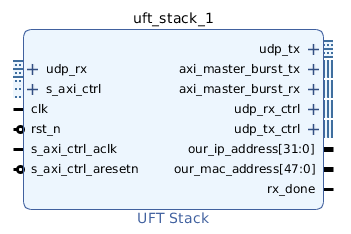
\includegraphics[width=0.5\textwidth] {images/dataflow/uftcoreaxilite.png}
    \caption{UFT core with AXI4-Lite interface}
    \label{fig:uftcoreaxilite}
\end{figure}

% ==============================================================================
%                             Data Interface
% ==============================================================================
\subsection{Data Interface}
The UFT core was in the first place intended for file based data transfer from
PC to FPGA and vice versa. This led to the decision to use memory mapped AXI
interface to store the received data and read the data to be sent. This made
sense with the UFT protocol being file oriented. In the progress of developing
the Wallis filter, a stream based approach was pursued to reduce latency and
memory usage. With the UFT core being memory based, a controller had to be
introduced to send the data from memory to the Wallis filter. Early tests
foreshowed that the UFT core with its memory based interface would be the
limiting member in the data processing chain. So the core's data interface was
rewritten to support AXI4-Stream for data receiving and sending.

For solution B, the two \texttt{axi\_master\_burst} blocks were removed and the
code of the \texttt{uft\_rx\_mem\_ctl} and \texttt{uft\_tx\_data\_assembler}
changed to directly connect the AXI4-Stream from the UDP stack to the outside.
Advantage of this solution is the reduced latency and less memory usage. One
downside is that the receiver is no longer able to reorder packets if they do
not arrive in order. As long as the application runs on a closed network it can
be assumed that packets will not change order.

\begin{figure}[b!]
    \centering
    \begin{adjustbox}{max width=\textwidth}
        % \tikzsetnextfilename{system-overview}
\begin{tikzpicture}[
    rounded corners=0mm,
    entity/.style={
        draw,
        minimum height=1.0cm,
        minimum width=3cm,
        fill=white,
        anchor=north west,
    },
    entityold/.style={
        draw=gray!60,
        minimum height=1.0cm,
        minimum width=3cm,
        fill=gray!20,
        anchor=north west,
    },
]
    %coordinates
    \coordinate (orig)      at (0,0);
    \coordinate (crx)       at (0,0);
    \coordinate (crxmem)    at (5,0);

    \coordinate (ctxctl)    at (0,-2.5);
    \coordinate (ctxcmd)    at (5,-3.5);
    \coordinate (ctxdat)    at (5,-5.5);
    \coordinate (ctxarb)    at (10,-4.5);
    \coordinate (caxilite)  at (-5,-2.5);

    \coordinate (ctxamb)    at (0,-5.5);
    \coordinate (crxamb)    at (10,0);
    %nodes

    \begin{pgfonlayer}{main}
        % entities
        \node[entity, label={uft\_rx}] (rx) at (crx) {};
        \node[entity, label={[name=rxl] uft\_rx\_mem\_ctl}] (rxmem) at (crxmem) {};

        \node[entity, label={[name=ltxctl] uft\_tx\_ctl}] (txctl) at (ctxctl) {};
        \node[entity, label={[name=txcal]uft\_tx\_cmd\_assembler}] (txcmd) at (ctxcmd) {};
        \node[entity, label={uft\_tx\_data\_assembler}] (txdat) at (ctxdat) {};
        \node[entity, label={uft\_tx\_arbiter}] (txarb) at (ctxarb) {};

        \node[entityold, label={axi\_master\_burst}] (ambrx) at (crxamb) {};
        \node[entityold, label={axi\_master\_burst}] (ambtx) at (ctxamb) {};

        % ports
        \path[draw,{Latex[length=2.5mm]}-] ($(rx.180) + (0,1/6)$) -- ($(rx.180) + (-1.0,1/6)$) node[anchor=east] {rx\_hdr};
        \path[draw=blue,line width=0.5mm,{Latex[length=2.5mm]}-] ($(rx.180) + (0,-1/6)$) -- ($(rx.180) + (-1.0,-1/6)$) node[anchor=east] {s\_axi};
        \path[draw,{Latex[length=2.5mm]}-] ($(txctl.180) + (0,0)$) -- ($(txctl.180) + (-1.0,0)$) node[anchor=east] {controll};

        \path[draw=blue,line width=0.5mm,-{Latex[length=2.5mm]}] ($(rxmem.0) + (0,0)$) -- ($(rxmem.0) + (6.5,0/6)$) node[anchor=west] {s\_axi\_rx};
        \path[draw,-{Latex[length=2.5mm]}] ($(txctl.0) + (0,3.5/10)$) -- ($(txctl.0) + (11.5,3.5/10)$) node[anchor=west] {tx\_hdr};
        \path[draw=red,line width=0.5mm,-{Latex[length=2.5mm]}] ($(txarb.0) + (0,0/10)$) -- ($(txarb.0) + (1.5,0/10)$) node[anchor=west] {s\_axi};

        % Interconnects
        \path[draw,-{Latex[length=2.5mm]}] ($(rx.0) + (0,1/6)$) -- ($(rxmem.180) + (0,1/6)$) node[anchor=east] {};
        \path[draw=blue,line width=0.5mm,-{Latex[length=2.5mm]}] ($(rx.0) + (0,-1/6)$) -- ($(rxmem.180) + (0,-1/6)$) node[midway, anchor=north] {s\_axi};
        % \node at ($(rx.180) + (-0.5,-1/6)$) [circle,fill,inner sep=1.5pt]{};

        \path[draw,-{Latex[length=2.5mm]}] ($(txctl.0) + (0,1.5/10)$) -| ($(txcmd.180) + (-0.5,0)$) -- ($(txcmd.180) + (0,0)$) node[anchor=west] {};
        \path[draw,-{Latex[length=2.5mm]}] ($(txctl.0) + (0,-1.5/10)$) -| ($(txarb.180) + (-6,0)$) -- ($(txarb.180) + (0,0)$) node[anchor=west] {};
        \path[draw,-{Latex[length=2.5mm]}] ($(txctl.0) + (0,-3.5/10)$) -| ($(txdat.180) + (-1.5,1/6)$) -- ($(txdat.180) + (0,1/6)$) node[anchor=west] {};

        \path[draw,-{Latex[length=2.5mm]}] ($(txcmd.0) + (0,0)$) -| node[anchor=south] {s\_axi} ($(txarb.180) + (-0.5,1/4)$)  -- ($(txarb.180) + (0,1/4)$);
        \path[draw=red,line width=0.5mm,-{Latex[length=2.5mm]}] ($(txdat.0) + (0,0)$) -| node[anchor=north] {s\_axi}($(txarb.180) + (-0.5,-1/4)$) -- ($(txarb.180) + (0,-1/4)$);

        \path[draw=red,line width=0.5mm,-{Latex[length=2.5mm]}] ($(txdat.180) + (-6,-1/6)$) node[anchor=east] {s\_axi\_tx} -- ($(txdat.180) + (0,-1/6)$) node[anchor=east] {};

        % Ack
        \path[draw,-{Latex[length=2.5mm]}] ($(crxmem.0) + (1.5,-1)$) |- ($(crxmem.0) + (-1,-2)$) -| ($(ctxctl.0) + (2.5,0)$) node[midway, anchor=east] {};


    \end{pgfonlayer}

    % tx box
    \begin{pgfonlayer}{foreground}
        \node [draw, fill=gray!20, inner sep=10, fit={(ltxctl) (txctl) (txcmd) (txdat) (txarb) (txcal)}, label={[label distance=0.0cm]150:uft\_tx\_top}] (tx) {};
    \end{pgfonlayer} 

    % Board box
    \begin{pgfonlayer}{background}
        \node [draw, fill=gray!40, inner sep=10, fit={(tx) (rx) (rxmem) (rxl)}, label=uft\_top] (tx) {};
    \end{pgfonlayer} 

\end{tikzpicture}
    \end{adjustbox}
    \caption{UFT Top Block Design with AXI4-Stram interface}
    \label{fig:ufttopstream}
\end{figure}

% ==============================================================================
%                             Implemented Features
% ==============================================================================
\clearpage
\subsection{Implemented Features}
In the final version of the UFT core used in solution B the AXI4-Lite interface
was removed because no memory addresses had to be exchanged and the solution B
controller was written in VHDL. Adding an AXI4-Lite master interface would have
only made it more complicated. 
\\

To conclude the changes made to the UFT core from the version of project 5:
\begin{itemize}
  \item Added acknowledgment on receiver path
  \item Changed data interfaces from memory mapped to AXI4-Stream
  \item Added user register to exchange configuration data
  \item Bug fixes
\end{itemize}

There are still some features that are not yet implemented but are defined in
the UFT protocol specifications:
\begin{itemize}
  \item Acknowledge and retransmission during send
\end{itemize}

Figure \ref{fig:uftipcoreaxistream} shows the IP core with the AXI4-Stream
ports.

\begin{figure}[b!]
    \centering
    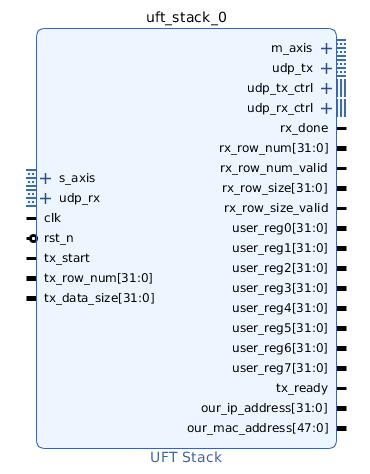
\includegraphics[width=0.5\textwidth] {images/dataflow/uftcorestream.png}
    \caption{UFT IP core with AXI4-Stream interface}
    \label{fig:uftipcoreaxistream}
\end{figure}
% ==============================================================================
%                             Control
% ==============================================================================
\section{Control} \label{ch:control}

% ==============================================================================
%                             Concept
% ==============================================================================
\subsection{Concept}

\subsection{Implementation (HLS)}


\subsubsection*{IF-Statement} \label{ch:data:if}

\begin{minipage}{\textwidth}
\begin{lstlisting}[style=CStyle, caption=Buffer switching reloading without else statement, label=lst:buf_false]
if( (outPpBuf == ppBufA) && (ms_pctr < (inLineSize-PIN_PONG_BUF_SIZE)) ) {
    if(!ppBufBrdy) {
        ...
    }
}
if( (outPpBuf == ppBufB) && (ms_pctr < (inLineSize-PIN_PONG_BUF_SIZE)) ) {
    if(!ppBufArdy) {
        ...
    }
}
\end{lstlisting}
\end{minipage}

\begin{minipage}{\textwidth}
\begin{lstlisting}[style=CStyle, caption=Buffer switching reloading with else statement, label=lst:buf_right]
if (ms_pctr < (inLineSize-PIN_PONG_BUF_SIZE)) {
	if( (outPpBuf == ppBufA)  ) {
		if(!ppBufBrdy) {
			...
		}
	}
	else {
		if(!ppBufArdy) {
			...
		}
	}
}
\end{lstlisting}
\end{minipage}

\subsection{Implementation (VHDL)}
